\usetikzlibrary{arrows.meta}
\graphicspath{{./figures/}}
\tikzset{|/.tip={Bar[width=.8ex,round]}}
\makeatletter
\newcommand{\diagdenomb}{\@ifstar{\@diagdenomb}{\@@diagdenomb}}
\newcommand{\@diagdenomb}{\begin{figure}[!htbp]
    \centering
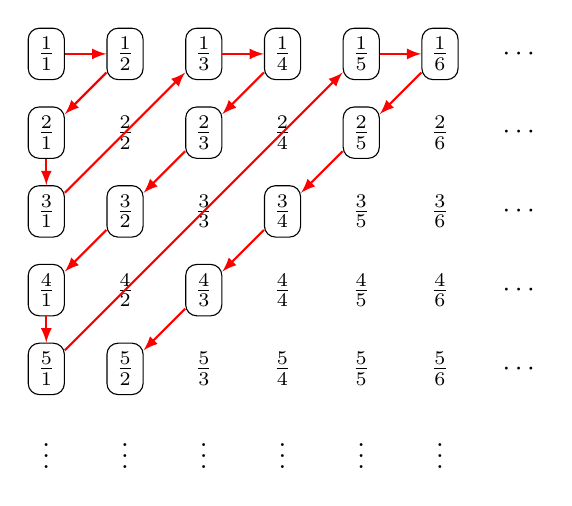
\begin{tikzpicture}
\tikzstyle{keepstyle} =[rectangle, rounded corners, draw, fill=white]
\node at (0,0) {$\vdots$};
\node[keepstyle] (51) at (0,1) {$\frac{5}{1}$};
\node[keepstyle] (41) at (0,2) {$\frac{4}{1}$};
\node[keepstyle] (31) at (0,3) {$\frac{3}{1}$};
\node[keepstyle] (21) at (0,4) {$\frac{2}{1}$};
\node[keepstyle] (11) at (0,5) {$\frac{1}{1}$};
\node at (1,0) {$\vdots$};
\node[keepstyle] (52) at (1,1) {$\frac{5}{2}$};
\node at (1,2) {$\frac{4}{2}$};
\node[keepstyle] (32) at (1,3) {$\frac{3}{2}$};
\node at (1,4) {$\frac{2}{2}$};
\node[keepstyle] (12) at (1,5) {$\frac{1}{2}$};
\node at (2,0) {$\vdots$};
\node at (2,1) {$\frac{5}{3}$};
\node[keepstyle] (43) at (2,2) {$\frac{4}{3}$};
\node at (2,3) {$\frac{3}{3}$};
\node[keepstyle] (23) at (2,4) {$\frac{2}{3}$};
\node[keepstyle] (13) at (2,5) {$\frac{1}{3}$};
\node at (3,0) {$\vdots$};
\node at (3,1) {$\frac{5}{4}$};
\node at (3,2) {$\frac{4}{4}$};
\node[keepstyle] (34) at (3,3) {$\frac{3}{4}$};
\node at (3,4) {$\frac{2}{4}$};
\node[keepstyle] (14) at (3,5) {$\frac{1}{4}$};
\node at (4,0) {$\vdots$};
\node  at (4,1) {$\frac{5}{5}$};
\node at (4,2) {$\frac{4}{5}$};
\node at (4,3) {$\frac{3}{5}$};
\node[keepstyle] (25) at (4,4) {$\frac{2}{5}$};
\node[keepstyle] (15) at (4,5) {$\frac{1}{5}$};
\node at (5,0) {$\vdots$};
\node  at (5,1) {$\frac{5}{6}$};
\node at (5,2) {$\frac{4}{6}$};
\node at (5,3) {$\frac{3}{6}$};
\node at (5,4) {$\frac{2}{6}$};
\node[keepstyle] (16) at (5,5) {$\frac{1}{6}$};
\node at (6,1) {$\cdots$};
\node at (6,2) {$\cdots$};
\node at (6,3) {$\cdots$};
\node at (6,4) {$\cdots$};
\node at (6,5) {$\cdots$};
\draw [-latex,red, thick] (11) -- (12);
\draw [-latex, red, thick] (12) -- (21);
\draw [-latex, red, thick] (21) -- (31);
\draw [-latex, red, thick] (31) -- (13);
\draw [-latex, red, thick] (13) -- (14);
\draw [-latex, red, thick] (14) -- (23);
\draw [-latex, red, thick] (23) -- (32);
\draw [-latex, red, thick] (32) -- (41);    
\draw [-latex, red, thick] (41) -- (51);
\draw [-latex, red, thick] (51) -- (15);
\draw [-latex, red, thick] (15) -- (16);
\draw [-latex, red, thick] (16) -- (25);
\draw [-latex, red, thick] (25) -- (34);
\draw [-latex, red, thick] (34) -- (43);
\draw [-latex, red, thick] (43) -- (52);
\end{tikzpicture}
\end{figure}
}
\newcommand{\@@diagdenomb}{\begin{figure}[htbp]
    \centering
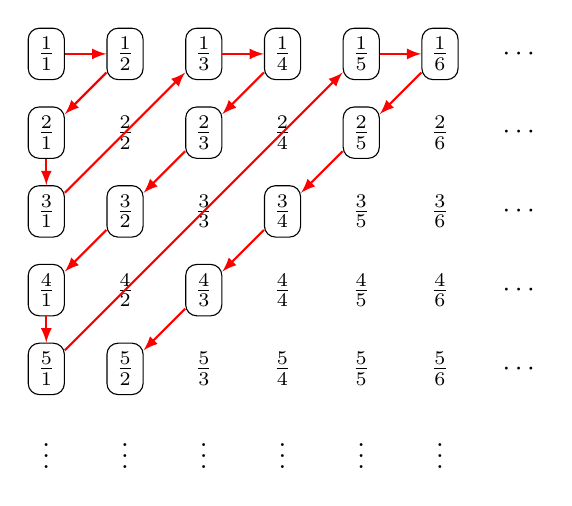
\begin{tikzpicture}
\tikzstyle{keepstyle} =[rectangle, rounded corners, draw, fill=white]
\node at (0,0) {$\vdots$};
\node[keepstyle] (51) at (0,1) {$\frac{5}{1}$};
\node[keepstyle] (41) at (0,2) {$\frac{4}{1}$};
\node[keepstyle] (31) at (0,3) {$\frac{3}{1}$};
\node[keepstyle] (21) at (0,4) {$\frac{2}{1}$};
\node[keepstyle] (11) at (0,5) {$\frac{1}{1}$};
\node at (1,0) {$\vdots$};
\node[keepstyle] (52) at (1,1) {$\frac{5}{2}$};
\node at (1,2) {$\frac{4}{2}$};
\node[keepstyle] (32) at (1,3) {$\frac{3}{2}$};
\node at (1,4) {$\frac{2}{2}$};
\node[keepstyle] (12) at (1,5) {$\frac{1}{2}$};
\node at (2,0) {$\vdots$};
\node at (2,1) {$\frac{5}{3}$};
\node[keepstyle] (43) at (2,2) {$\frac{4}{3}$};
\node at (2,3) {$\frac{3}{3}$};
\node[keepstyle] (23) at (2,4) {$\frac{2}{3}$};
\node[keepstyle] (13) at (2,5) {$\frac{1}{3}$};
\node at (3,0) {$\vdots$};
\node at (3,1) {$\frac{5}{4}$};
\node at (3,2) {$\frac{4}{4}$};
\node[keepstyle] (34) at (3,3) {$\frac{3}{4}$};
\node at (3,4) {$\frac{2}{4}$};
\node[keepstyle] (14) at (3,5) {$\frac{1}{4}$};
\node at (4,0) {$\vdots$};
\node  at (4,1) {$\frac{5}{5}$};
\node at (4,2) {$\frac{4}{5}$};
\node at (4,3) {$\frac{3}{5}$};
\node[keepstyle] (25) at (4,4) {$\frac{2}{5}$};
\node[keepstyle] (15) at (4,5) {$\frac{1}{5}$};
\node at (5,0) {$\vdots$};
\node  at (5,1) {$\frac{5}{6}$};
\node at (5,2) {$\frac{4}{6}$};
\node at (5,3) {$\frac{3}{6}$};
\node at (5,4) {$\frac{2}{6}$};
\node[keepstyle] (16) at (5,5) {$\frac{1}{6}$};
\node at (6,1) {$\cdots$};
\node at (6,2) {$\cdots$};
\node at (6,3) {$\cdots$};
\node at (6,4) {$\cdots$};
\node at (6,5) {$\cdots$};
\draw [-latex,red, thick] (11) -- (12);
\draw [-latex, red, thick] (12) -- (21);
\draw [-latex, red, thick] (21) -- (31);
\draw [-latex, red, thick] (31) -- (13);
\draw [-latex, red, thick] (13) -- (14);
\draw [-latex, red, thick] (14) -- (23);
\draw [-latex, red, thick] (23) -- (32);
\draw [-latex, red, thick] (32) -- (41);    
\draw [-latex, red, thick] (41) -- (51);
\draw [-latex, red, thick] (51) -- (15);
\draw [-latex, red, thick] (15) -- (16);
\draw [-latex, red, thick] (16) -- (25);
\draw [-latex, red, thick] (25) -- (34);
\draw [-latex, red, thick] (34) -- (43);
\draw [-latex, red, thick] (43) -- (52);
\end{tikzpicture}
\caption{Dénombrabilité de $\mathbb{Q}$\protect\cite{Tikz-Count}}
    \label{fig:denombQ}
\end{figure}
}
\tikzset{    >=stealth,
    bullet/.style={
        fill=black,
        circle,
        minimum width=1pt,
        inner sep=1pt
    },
    projection/.style={
        thick,
        shorten <=2pt,
        shorten >=2pt
    },
    every fit/.style={
        ellipse,
        draw,
        inner sep=2pt
        }}
\makeatother
\graphicspath{{./figures/}} % pour les images, plus besoin d'écrire "./figures"
\newcommand{\diagfonctbij}{
	\begin{figure}[htbp]
	\centering
    \begin{tikzpicture}
	\node[bullet,fill=bleu,label=left:$a$] (a1) at (0,4) {};    
	\node[bullet,fill=bleu,label=left:$b$] (a2) at (0,3) {};    
	\node[bullet,fill=bleu,label=left:$c$] (a3) at (0,2) {};
	\node[bullet,fill=bleu,label=left:$d$] (a4) at (0,1) {};%
	%
	\node[bullet,fill=roug,label=right:$1$] (b1) at (4,4) {};
	\node[bullet,fill=roug,label=right:$2$] (b2) at (4,3) {};
	\node[bullet,fill=roug,label=right:$3$] (b3) at (4,2) {};
	\node[bullet,fill=roug,label=right:$4$] (b4) at (4,1) {};%
%
	\node[fill=bleu,draw=bleu,fill opacity=0.3,fit= (a1) (a2) (a3) (a4),minimum width=2cm, label=above:$E$] (X) {} ;
	\node[fill=roug,draw=roug,fill opacity=0.3,fit= (b1) (b2) (b3) (b4),minimum width=2cm, label=above:$F$] (Y) {} ;  %
%
	\draw[|->,projection] (a1) to[out=20, in=150] (b4);
	\draw[|->,projection] (a2) to[out=20, in=160] (b2);
	\draw[|->,projection] (a3) to[out=20, in=170] (b1);
	\draw[|->,projection] (a4) to[out=20, in=150] (b3);
%
	\draw[->,thick,shorten <=1cm,shorten >=1cm] (X.north) -- node [midway,above,align=center]{$f$} (Y.north);
	\end{tikzpicture}%
%
	\caption{diagramme sagittal d'une application bijective.}
	\label{fig:fonctbij}
\end{figure}
}
\newcommand{\diagfonctinj}{
	\begin{figure}[htbp]
	\centering
    \begin{tikzpicture}
	\node[bullet,fill=bleu,label=left:$a$] (a1) at (0,4) {};    
	\node[bullet,fill=bleu,label=left:$b$] (a2) at (0,3) {};    
	\node[bullet,fill=bleu,label=left:$c$] (a3) at (0,2) {};%
	%
	\node[bullet,fill=roug,label=right:$1$] (b1) at (4,4) {};
	\node[bullet,fill=roug,label=right:$2$] (b2) at (4,3) {};
	\node[bullet,fill=roug,label=right:$3$] (b3) at (4,2) {};
	\node[bullet,fill=roug,label=right:$4$] (b4) at (4,1) {};%
%
	\node[fill=bleu,draw=bleu,fill opacity=0.3,fit= (a1) (a2) (a3),minimum width=2cm, label=above:$X$] (X) {} ;
	\node[fill=roug,draw=roug,fill opacity=0.3,fit= (b1) (b2) (b3) (b4),minimum width=2cm, label=above:$Y$] (Y) {} ;  %
%
	\draw[|->,projection] (a1) to[out=20, in=150] (b4);
	\draw[|->,projection] (a2) to[out=20, in=160] (b2);
	\draw[|->,projection] (a3) to[out=20, in=170] (b1);
%
	\draw[->,thick,shorten <=1cm,shorten >=1cm] (X.north) -- node [midway,above,align=center]{$f$} (Y.north);
	\end{tikzpicture}%
%
	\caption{diagramme sagittal d'une application injective.}
	\label{fig:fonctinj}
\end{figure}
}
\newcommand{\diagfonctsurj}{
	\begin{figure}[htbp]
	\centering
    \begin{tikzpicture}
	\node[bullet,fill=bleu,label=left:$a$] (a1) at (0,4) {};    
	\node[bullet,fill=bleu,label=left:$b$] (a2) at (0,3) {};    
	\node[bullet,fill=bleu,label=left:$c$] (a3) at (0,2) {};%
	\node[bullet,fill=bleu,label=left:$c$] (a4) at (0,1) {};%
	%
	\node[bullet,fill=roug,label=right:$1$] (b1) at (4,4) {};
	\node[bullet,fill=roug,label=right:$2$] (b2) at (4,3) {};
	\node[bullet,fill=roug,label=right:$3$] (b3) at (4,2) {};
%
	\node[fill=bleu,draw=bleu,fill opacity=0.3,fit= (a1) (a2) (a3) (a4),minimum width=2cm, label=above:$X$] (X) {} ;
	\node[fill=roug,draw=roug,fill opacity=0.3,fit= (b1) (b2) (b3),minimum width=2cm, label=above:$Y$] (Y) {} ;  %
%
	\draw[|->,projection] (a1) to[out=20, in=150] (b3);
	\draw[|->,projection] (a2) to[out=20, in=160] (b2);
	\draw[|->,projection] (a3) to[out=20, in=170] (b1);
	\draw[|->,projection] (a4) to[out=20, in=170] (b1);
%
	\draw[->,thick,shorten <=1cm,shorten >=1cm] (X.north) -- node [midway,above,align=center]{$f$} (Y.north);
	\end{tikzpicture}%
%
	\caption{diagramme sagittal d'une application surjective.\\ On a $|X|\geq|Y|$.}
	\label{fig:fonctsurj}
\end{figure}
}
\newcommand{\diagcompfonct}{
	\begin{figure}[htbp]
		\centering
		\begin{tikzpicture}
			\node[bullet,label=left:$a$] (a1) at (0,4) {};    
			\node[coordinate,label] (a2) at (0,3) {};    
			\node[coordinate,label] (a3) at (0,2) {};
			\node[coordinate,label] (a4) at (0,1) {};
			\node[coordinate,fill=roug] (b1) at (4,4) {};
			\node[coordinate,fill=roug] (b2) at (4,3) {};
			\node[coordinate,fill=roug] (b3) at (4,2) {};
			\node[bullet,fill=roug,label=right:$4$] (b4) at (4,1) {};
			\node[coordinate,fill=vert] (c1) at (8,4) {};
			\node[bullet,fill=vert,label=right:pair] (c2) at (8,3) {};
			\node[coordinate,fill=vert] (c3) at (8,2) {};
			\node[coordinate,fill=vert] (c4) at (8,1) {};
			\node[fill=bleu,draw=bleu,fill opacity=0.3,fit= (a1) (a2) (a3) (a4),minimum width=2cm, label=above:$X$] (X) {} ;
			\node[fill=roug,draw=roug,fill opacity=0.3,fit= (b1) (b2) (b3) (b4),minimum width=2cm, label=above:$Y$] (Y) {} ;  
			\node[fill=vert,draw=vert,fill opacity=0.3,fit= (c1) (c2) (c3) (c4),minimum width=2cm, label=above:$Z$] (Z) {} ;  
			\draw[|->,projection] (a1) to[out=-10, in=150] (b4);
			%
			\draw[|->,projection] (b4) to[out=50, in=180] (c2);
			\draw[|->,projection,dashed] (a1) to[out=-25, in=180] (c2);
			%
			\draw[->,thick,shorten <=1cm,shorten >=1cm] (X.north) -- node [midway,above,align=center]{$f$} (Y.north);
			\draw[->,thick,shorten <=1cm,shorten >=1cm] (Y.north) -- node [midway,above,align=center]{$g$} (Z.north);
			\draw[->,thick,dashed,shorten <=.5cm,shorten >=.5cm] (X.north) to[out=50, in=130] node [midway,above=.25em,align=center]{$g\circ f$} (Z.north);
		\end{tikzpicture}
		\caption{Composition d'applications, détail pour un antécédent.}
		\label{fig:diagcompfonct}
	\end{figure}
}